\documentclass[a4paper]{article}

%% Language and font encodings
\usepackage[english]{babel}
\usepackage[utf8]{inputenc}
\usepackage[T1]{fontenc}
\usepackage[section]{placeins}
\usepackage{graphicx}
\usepackage{caption}
\usepackage{subcaption}
\usepackage{float}
\usepackage{verbatim}
\usepackage{color,soul}
\usepackage[backend=biber,style=ieee]{biblatex}
\addbibresource{main.bib}


%% Sets page size and margins
\usepackage[a4paper,top=3cm,bottom=2cm,left=3cm,right=3cm,marginparwidth=1.75cm]{geometry}

%% Useful packages
\usepackage{amsmath}
\usepackage{graphicx}
\usepackage[colorinlistoftodos]{todonotes}
\usepackage[colorlinks=true, allcolors=blue]{hyperref}
\usepackage{listings}
\usepackage{color} %red, green, blue, yellow, cyan, magenta, black, white
\definecolor{mygreen}{RGB}{28,172,0} % color values Red, Green, Blue
\definecolor{mylilas}{RGB}{170,55,241}

\makeatletter
\newcommand{\filecaption}[1]{\filename@parse{#1}\filename@base.\filename@ext}
\makeatother

\newcommand{\filelisting}[2][]{%
	\lstinputlisting[caption={\texttt{\protect\filecaption{\detokenize{#2}}}},#1]{#2}%
}

\newcommand{\code}[1]{\texttt{\detokenize{#1}}}

\title{ECE 271 Design Project, Group 3}
\author{Casey Huggins, Raymond Jung, Matthew Macovsky, Patrick McGrath}
\date{June 6th, 2019}

\begin{document}

\lstset{language=Verilog,%
    basicstyle=\tiny \color{red},
    breaklines=true,%
    keywordstyle=\color{blue},%
    morekeywords=[2]{1}, keywordstyle=[2]{\color{black}},
    identifierstyle=\color{black},%
    stringstyle=\color{mylilas},
    commentstyle=\color{mygreen},%
    showstringspaces=false,%without this there will be a symbol in the places where there is a space
    numbers=left,%
    numberstyle={\tiny \color{black}},% size of the numbers
    numbersep=9pt, % this defines how far the numbers are from the text
    emph=[1]{for,end,break},emphstyle=[1]\color{red}, %some words to emphasise
    %title=\lstname
}

\maketitle
\tableofcontents
\newpage
\section{Project Description}

\newpage
\section{High Level Description}

TODO

\begin{figure}[ht]
  \centering
    
\includegraphics[width=.5\textwidth]{images/block_diagrams/top_level.png}
	\caption{The top level design for this project.}
    \label{fig:top_level}
\end{figure}


\subsection{NES Controller Reader}
\subsubsection{Individual Block}
\subsubsection{Next Individual Block}
\subsubsection{Next Individual Block}
\subsubsection{Next Individual Block}
\subsubsection{Next Individual Block}

\subsection{PS2 Keyboard Decoder}
\subsubsection{Individual Block}
\subsubsection{Next Individual Block}
\subsubsection{Next Individual Block}
\subsubsection{Next Individual Block}
\subsubsection{Next Individual Block}

\subsection{VCR Remote Decoder}

\textbf{Input:} This reads a 50MHz clock signal (\code{i_clk}), an active low reset (\code{i_reset_n}), and a signal from an IR sensor (\code{i_ir_signal}).
\\ \\
\textbf{Output:} \code{o_button_ss[6..0]} is used to display the latest VCR remote button value received on a 7-segment display.  This output also turns the display off if no code has yet been recieved or an unrecognized code was received.  \code{o_checksum_valid} indicates whether the latest 32-bit code received has a vaild checksum, which is be the case for all valid codes.
\\ \\
The code for this block is given in \autoref{lst:sv_vcr_ir_decoder}.

\begin{figure}[H]
  \centering
    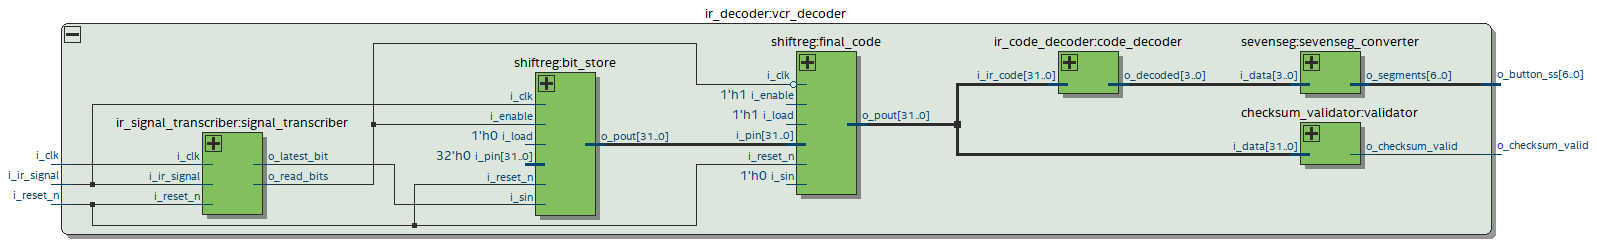
\includegraphics[width=.85\textwidth]{images/block_diagrams/vcr_remote/ir_decoder.png}
	\caption{An expanded view of the top-level VCR remote decoder block in \autoref{fig:top_level}.  This interprets codes sent over IR using the NEC protocol as described in \cite{nec}.  A signal transcriber (\code{signal_transcriber}) determines whether bits are currently being sent and the most recent bit.  These are fed into a shift register (\code{bit_store}) at the end of the transmission of each bit.  Once an entire code has been transmitted, the contents of that register are transferred to another, \code{final_code}.  The checksum of this code is then checked by the checksum validator \code{validator} and output to \code{o_checksum_valid}.  It is also decoded to the number pressed on the remote by a decoder (\code{code_decoder}) and then converted to a 7-segment display signal by \code{segsev_converter} before being output to \code{o_button_ss}.}
    \label{fig:block_vcr_ir_decoder}
\end{figure}

\begin{figure}[H]
	\centering
	\includegraphics[width=.8\textwidth]{images/sim/vcr_remote/0.png}
	\caption{Simulation results for a "0" signal (see \autoref{lst:sim_vcr_ir_decoder_0} for simulation code).}
\end{figure}

\begin{figure}[H]
	\centering
	\includegraphics[width=.8\textwidth]{images/sim/vcr_remote/1.png}
	\caption{Simulation results for a "1" signal (see \autoref{lst:sim_vcr_ir_decoder_1} for simulation code).}
\end{figure}

\begin{figure}[H]
	\centering
	\includegraphics[width=.8\textwidth]{images/sim/vcr_remote/2.png}
	\caption{Simulation results for a "2" signal (see \autoref{lst:sim_vcr_ir_decoder_2} for simulation code).}
\end{figure}

\begin{figure}[H]
	\centering
	\includegraphics[width=.8\textwidth]{images/sim/vcr_remote/3.png}
	\caption{Simulation results for a "3" signal (see \autoref{lst:sim_vcr_ir_decoder_3} for simulation code).}
\end{figure}

\begin{figure}[H]
	\centering
	\includegraphics[width=.8\textwidth]{images/sim/vcr_remote/4.png}
	\caption{Simulation results for a "4" signal (see \autoref{lst:sim_vcr_ir_decoder_4} for simulation code).}
\end{figure}

\begin{figure}[H]
	\centering
	\includegraphics[width=.8\textwidth]{images/sim/vcr_remote/5.png}
	\caption{Simulation results for a "5" signal (see \autoref{lst:sim_vcr_ir_decoder_5} for simulation code).}
\end{figure}

\begin{figure}[H]
	\centering
	\includegraphics[width=.8\textwidth]{images/sim/vcr_remote/6.png}
	\caption{Simulation results for a "6" signal (see \autoref{lst:sim_vcr_ir_decoder_6} for simulation code).}
\end{figure}

\begin{figure}[H]
	\centering
	\includegraphics[width=.8\textwidth]{images/sim/vcr_remote/7.png}
	\caption{Simulation results for a "7" signal (see \autoref{lst:sim_vcr_ir_decoder_7} for simulation code).}
\end{figure}

\begin{figure}[H]
	\centering
	\includegraphics[width=.8\textwidth]{images/sim/vcr_remote/8.png}
	\caption{Simulation results for a "8" signal (see \autoref{lst:sim_vcr_ir_decoder_8} for simulation code).}
\end{figure}

\begin{figure}[H]
	\centering
	\includegraphics[width=.8\textwidth]{images/sim/vcr_remote/9.png}
	\caption{Simulation results for a "9" signal (see \autoref{lst:sim_vcr_ir_decoder_9} for simulation code).}
\end{figure}

\begin{figure}[H]
	\centering
	\includegraphics[width=.8\textwidth]{images/sim/vcr_remote/sequence.png}
	\caption{Simulation results for a "1" signal followed by a "2" signal (see \autoref{lst:sim_vcr_ir_decoder_sequence} for simulation code).}
\end{figure}

\begin{figure}[H]
	\centering
	\includegraphics[width=.8\textwidth]{images/sim/vcr_remote/bad_checksum.png}
	\caption{Simulation results for a signal producing an invalid code (see \autoref{lst:sim_vcr_ir_decoder_bad_checksum} for simulation code).}
\end{figure}

\subsubsection{IR Signal Transcriber}

\textbf{Input:} This reads a 50MHz clock signal (\code{i_clk}), an active low reset (\code{i_reset_n}), and a signal from an IR sensor (\code{i_ir_signal}).
\\ \\
\textbf{Output:} \code{o_latest_bit} indicates the last bit seen in the IR signal.  \code{o_read_bits} indicates whether new bits are currently being read.
\\ \\
The code for this block is given in \autoref{lst:sv_vcr_ir_signal_transcriber}.
\\ \\
The simulations in the previous section also serve to simulate this module.

\begin{figure}[H]
  \centering
    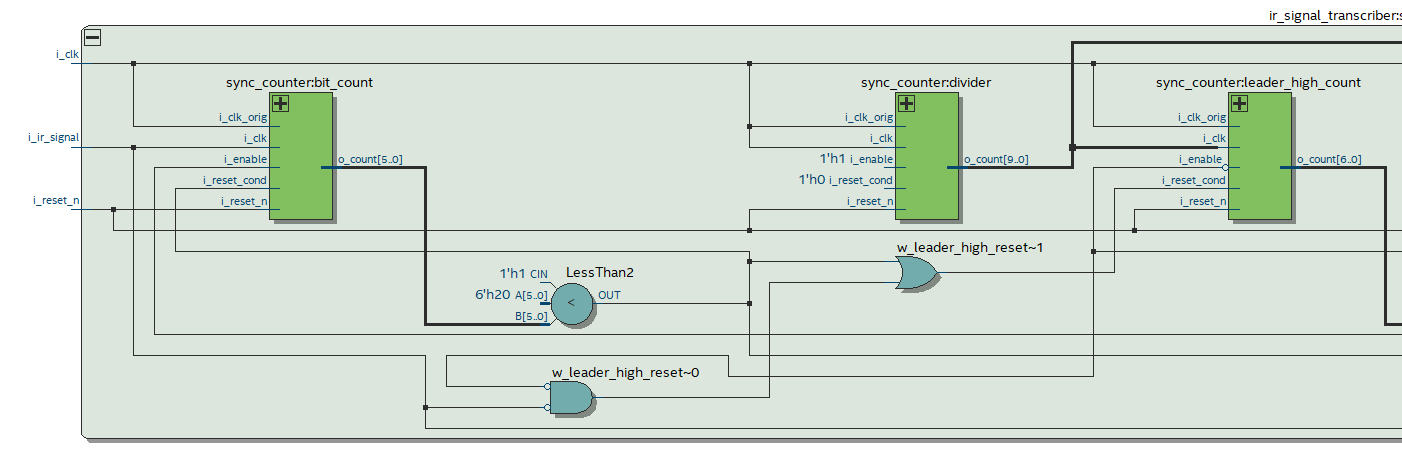
\includegraphics[width=.85\textwidth]{images/block_diagrams/vcr_remote/ir_signal_transcriber_1.png}
	\caption{An expanded view of the first half of the IR signal transcriber block in \autoref{fig:block_vcr_ir_decoder}.  A 10-bit counter (\code{divider}) divides the 10MHz input clock down to 10KHz.  Another counter, \code{leader_high_count}, uses this clock to count up as long as the input signal is high (for the high part of the leader) and it hasn't reached the length of that high part.  It resets if the signal goes low again before it has reached that value and when 32 bits have been read.  The bit counter to the left is enabled when the entire leader has ended and increments for each bit read.  It also resets when 32 bits have been read.}
    \label{fig:block_vcr_ir_signal_transcriber_1}
\end{figure}

\begin{figure}[H]
  \centering
    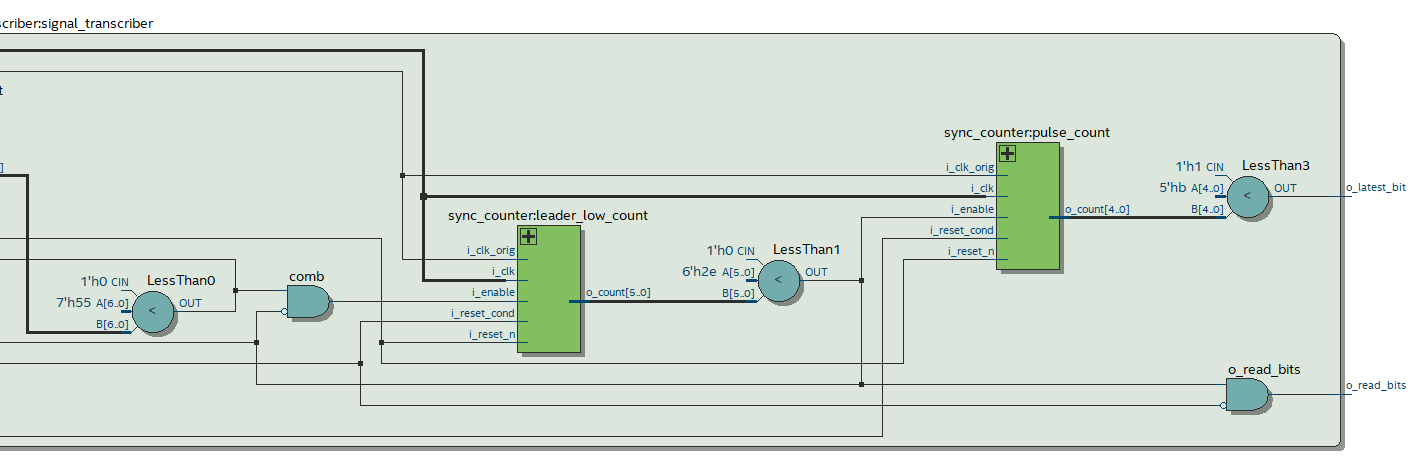
\includegraphics[width=.85\textwidth]{images/block_diagrams/vcr_remote/ir_signal_transcriber_2.png}
	\caption{An expanded view of the second half of the IR signal transcriber block in \autoref{fig:block_vcr_ir_decoder}.  A counter (\code{leader_low_count}) acts similarly to \code{leader_high_count}.  It is enabled when the high part of the leader has ended and counts up to the length of the low part of the leader.  It resets once it has reached that length.  At this point, \code{pulse_count} is enabled and counts as long as the signal is low.  This is used to determine the length of each pulse distance.  A comparator determines if the distance is less than a cutoff (a 0) or greater than the cutoff (signifying  a 1).  Additionally, \code{o_read_bits} is set high when the low part of the leader has ended and fewer than 32 bits have been read.}
    \label{fig:block_vcr_ir_signal_transcriber_2}
\end{figure}

\appendix
\section{SystemVerilog Files}
\filelisting[label=lst:sv_toplevel]{../verilog/final_project.sv}
\filelisting[label=lst:sv_devices_mux]{../verilog/devices_mux.sv}

\subsection{NES Controller Reader}
TODO

\subsection{PS2 Keyboard Decoder}
TODO

\subsection{VCR Remote Decoder}
\filelisting[label=lst:sv_vcr_ir_decoder]{../verilog/vcr_remote/ir_decoder.sv}
\filelisting[label=lst:sv_vcr_ir_signal_transcriber]{../verilog/vcr_remote/ir_signal_transcriber.sv}
\filelisting[label=lst:sv_vcr_sync_counter]{../verilog/vcr_remote/sync_counter.sv}
\filelisting[label=lst:sv_vcr_counter]{../verilog/vcr_remote/counter.sv}
\filelisting[label=lst:sv_vcr_sync]{../verilog/vcr_remote/sync.sv}
\filelisting[label=lst:sv_vcr_shiftreg]{../verilog/vcr_remote/shiftreg.sv}
\filelisting[label=lst:sv_vcr_checksum_validator]{../verilog/vcr_remote/checksum_validator.sv}
\filelisting[label=lst:sv_vcr_ir_code_decoder]{../verilog/vcr_remote/ir_code_decoder.sv}

\section{Simulation Files (Do scripts)}

\subsection{NES Controller Reader}
TODO

\subsection{PS2 Keyboard Decoder}
TODO

\subsection{VCR Remote Decoder}

\subsubsection{ir\_decoder Module}
\filelisting[float]{../do_files/vcr_remote/setup.do}
\filelisting[float]{../do_files/vcr_remote/reset.do}
\filelisting[float,label=lst:sim_vcr_ir_decoder_0]{../do_files/vcr_remote/0.do}
\filelisting[float,label=lst:sim_vcr_ir_decoder_1]{../do_files/vcr_remote/1.do}
\filelisting[float,label=lst:sim_vcr_ir_decoder_2]{../do_files/vcr_remote/2.do}
\filelisting[float,label=lst:sim_vcr_ir_decoder_3]{../do_files/vcr_remote/3.do}
\filelisting[float,label=lst:sim_vcr_ir_decoder_4]{../do_files/vcr_remote/4.do}
\filelisting[float,label=lst:sim_vcr_ir_decoder_5]{../do_files/vcr_remote/5.do}
\filelisting[float,label=lst:sim_vcr_ir_decoder_6]{../do_files/vcr_remote/6.do}
\filelisting[float,label=lst:sim_vcr_ir_decoder_7]{../do_files/vcr_remote/7.do}
\filelisting[float,label=lst:sim_vcr_ir_decoder_8]{../do_files/vcr_remote/8.do}
\filelisting[float,label=lst:sim_vcr_ir_decoder_9]{../do_files/vcr_remote/9.do}
\filelisting[float,label=lst:sim_vcr_ir_decoder_sequence]{../do_files/vcr_remote/sequence.do}
\filelisting[float,label=lst:sim_vcr_ir_decoder_bad_checksum]{../do_files/vcr_remote/bad_checksum.do}

\printbibliography

\end{document}